% Options for packages loaded elsewhere
\PassOptionsToPackage{unicode}{hyperref}
\PassOptionsToPackage{hyphens}{url}
%
\documentclass[
]{article}
\usepackage{lmodern}
\usepackage{amssymb,amsmath}
\usepackage{ifxetex,ifluatex}
\ifnum 0\ifxetex 1\fi\ifluatex 1\fi=0 % if pdftex
  \usepackage[T1]{fontenc}
  \usepackage[utf8]{inputenc}
  \usepackage{textcomp} % provide euro and other symbols
\else % if luatex or xetex
  \usepackage{unicode-math}
  \defaultfontfeatures{Scale=MatchLowercase}
  \defaultfontfeatures[\rmfamily]{Ligatures=TeX,Scale=1}
\fi
% Use upquote if available, for straight quotes in verbatim environments
\IfFileExists{upquote.sty}{\usepackage{upquote}}{}
\IfFileExists{microtype.sty}{% use microtype if available
  \usepackage[]{microtype}
  \UseMicrotypeSet[protrusion]{basicmath} % disable protrusion for tt fonts
}{}
\makeatletter
\@ifundefined{KOMAClassName}{% if non-KOMA class
  \IfFileExists{parskip.sty}{%
    \usepackage{parskip}
  }{% else
    \setlength{\parindent}{0pt}
    \setlength{\parskip}{6pt plus 2pt minus 1pt}}
}{% if KOMA class
  \KOMAoptions{parskip=half}}
\makeatother
\usepackage{xcolor}
\IfFileExists{xurl.sty}{\usepackage{xurl}}{} % add URL line breaks if available
\IfFileExists{bookmark.sty}{\usepackage{bookmark}}{\usepackage{hyperref}}
\hypersetup{
  hidelinks,
  pdfcreator={LaTeX via pandoc}}
\urlstyle{same} % disable monospaced font for URLs
\usepackage{graphicx,grffile}
\makeatletter
\def\maxwidth{\ifdim\Gin@nat@width>\linewidth\linewidth\else\Gin@nat@width\fi}
\def\maxheight{\ifdim\Gin@nat@height>\textheight\textheight\else\Gin@nat@height\fi}
\makeatother
% Scale images if necessary, so that they will not overflow the page
% margins by default, and it is still possible to overwrite the defaults
% using explicit options in \includegraphics[width, height, ...]{}
\setkeys{Gin}{width=\maxwidth,height=\maxheight,keepaspectratio}
% Set default figure placement to htbp
\makeatletter
\def\fps@figure{htbp}
\makeatother
\setlength{\emergencystretch}{3em} % prevent overfull lines
\providecommand{\tightlist}{%
  \setlength{\itemsep}{0pt}\setlength{\parskip}{0pt}}
\setcounter{secnumdepth}{-\maxdimen} % remove section numbering

\date{}

\documentclass[11pt]{article} 
\begin{document}

\title{Assignment 3}
\author{Raymond Baker}
\date{\today}

\includegraphics[width=\columnwidth]{ryerson_logo.png}

\begin{flushleft}
\begin{tabular}{|p{0.4\textwidth}|p{0.6\textwidth}|} 
 \hline
    Course Title: & Digital Image Processing \\ [5ex]
 \hline
    Course Number: & ELE 882 \\ [5ex]
 \hline
    Semester/Year & Fall/2019 \\ [5ex]
 \hline

\end{tabular}
\end{flushleft}

\begin{flushleft}
\begin{tabular}{|p{0.4\textwidth}|p{0.6\textwidth}|} 
 \hline
    Instructor: & Ling Guan \\ [5ex]
 \hline
\end{tabular}
\end{flushleft}

\begin{flushleft}
\begin{tabular}{|p{0.4\textwidth}|p{0.6\textwidth}|} 
 \hline
    Assignment/Lab Number: & 3 \\[5ex]
 \hline
    Assignment/Lab Title: & Assignment 3 \\[5ex]
 \hline
\end{tabular}
\end{flushleft}

\begin{flushleft}
\begin{tabular}{|p{0.4\textwidth}|p{0.6\textwidth}|} 
 \hline
    Submission Date: & \today \\[5ex]
 \hline
    Due Date: & \today \\[5ex]
 \hline
\end{tabular}
\end{flushleft}

\begin{flushleft}
\begin{tabular}{|p{0.2\textwidth}|p{0.2\textwidth}|p{0.22\textwidth}|p{0.09\textwidth}|p{0.19\textwidth}|}
 \hline
     Student \linebreak LAST Name & Student \linebreak FIRST Name & Student \linebreak Number & Section & Signature* \\
 \hline
    Baker & Raymond & 500691429 & 03 & R.B. \\[5ex]
 \hline
    Bao & Doan & 500733516 & 03 & B.D. \\[5ex]
 \hline
\end{tabular}
\end{flushleft}

\pagebreak
\textbf{Introduction}

Throughout the lab, various forms of image enhancement was examined. These include histogram equalize, adaptive equalize, Laplacian sharpen, and the unsharp mask. An additional enhancement of the adaptive equalize will also be examined where a 'cutoff' parameter is included. The input of the histogram equalization will use the image as a whole, and attempt to create a uniform PDF for all intensity values. The adaptive equalization is a localized version of the global equalization where the input is only a window of the image. Both of these image enhancement types aim to improve the contrast of the image.

While these two aim to improve the contrast of the image, the unsharp mask and Laplacian sharpen aim to improve the sharpness of the image, increasing the emphasis on the edges. The unsharp mask is performed by the following steps: the image is first blurred through the Gaussian filter, then the difference of the original image with the blurred image is calculated and added back to the original image multiplied by a constant 'k'. By varying 'k', the strength of the unsharp mask can be modified. An additional parameter is the radius in which the Gaussian filter is calculated for. By increasing the radius, more neighboring pixels are considered for the Gaussian blur. However, as a result of this, the operation is more computationally expensive.

\pagebreak

\textbf{Analysis}

\textbf{Question 1}

What type of low-pass filter was best suited for handling additive noise? What type of filter was best suited for multiplicative noise? Salt and pepper? Explain why based on your results.

To mitigate the effects of salt and pepper the best filter is the median. For multiplicative noise, a Gaussian filter was used to lessen the effects of noise.
 
\textbf{Question 2}

Consider the how the different types of noise are defined. Theoretically, what type of filters would be best suited for removing the different noise types. Compare this to the results that you obtained.

Salt and pepper is best solved with a median filter. 

Additive noise has a Gaussian form, as such, applying a Gaussian filter to it should result in reduced image.

\textbf{Question 3}

 Compare and contrast the global histogram equalization to the local histogram equalization. Are there any circumstances where the global method is better? The local method?
 
 The global histogram equalization takes into account a full image whereas the local histogram equalization only looks at a window. The result of the local histogram equalization may result in a tiled effect, however, this can be beneficial if the image has different regions of varying intensity. For example, a very dark background and a very bright foreground.

\textbf{Question 4}

You implemented two types of sharpening operators: unsharp masking and Laplacian sharpening. Compare and contrast the two method. Is one better? Why or why not? Ignore the fact that Laplacian sharpening is computationally simpler.

The unsharp takes the low freq components of the image and does a weighted subtraction them from the original image. While the Laplacian takes the increases the contrast between the two sides of an edge. 

\textbf{Question 5}

Based on your results, what is the benefit to the clamping done by the CLAHE method? Earlier in this document it was stated that this helps to avoid boosting noise in regions of uniform value. Why, or why not, would this be the case?

The CLAHE method results in a more even distribution of intensity values. An issue with the local histogram equalization is that it amplifies noise. The noise is boosted in regions of uniform value due to the CDF. By applying the CLAHE method, the areas of uniform intensity are redistributed. This results in a weaker effect from noise.

\pagebreak

\textbf{Conclusion}

After examining the different forms of image enhancement, the following was found. When comparing global histogram equalization to local histogram equalization, it was found that the local histogram equalization performed better where the image contained regions of low contrast. When examining the two operators which sharpened the image, Laplacian sharpening and unsharp masking, it was seen that the Laplacian sharpening operator increases the contrast between two edges, whereas the unsharp mask only took into account the low frequency components of the image.  

\pagebreak

\textbf{2.1.1 Q1 - Global Histogram Equalization}
\begin{verbatim}
function out = histogram_equalize(img)
    out = img;
    total_count = size(img, 1) * size(img, 2);
    if ~(isa(img, 'uint8'))
        disp ('Invalid Type');
        out = 1;
    else
        for i = 0:255
            new_val = floor((length(img(img <= i))/total_count)*255);
            out(img==i) = new_val;
        end
    end
end

imshow(histogram_equalize(a));
imshow(histogram_equalize(b));

\end{verbatim}

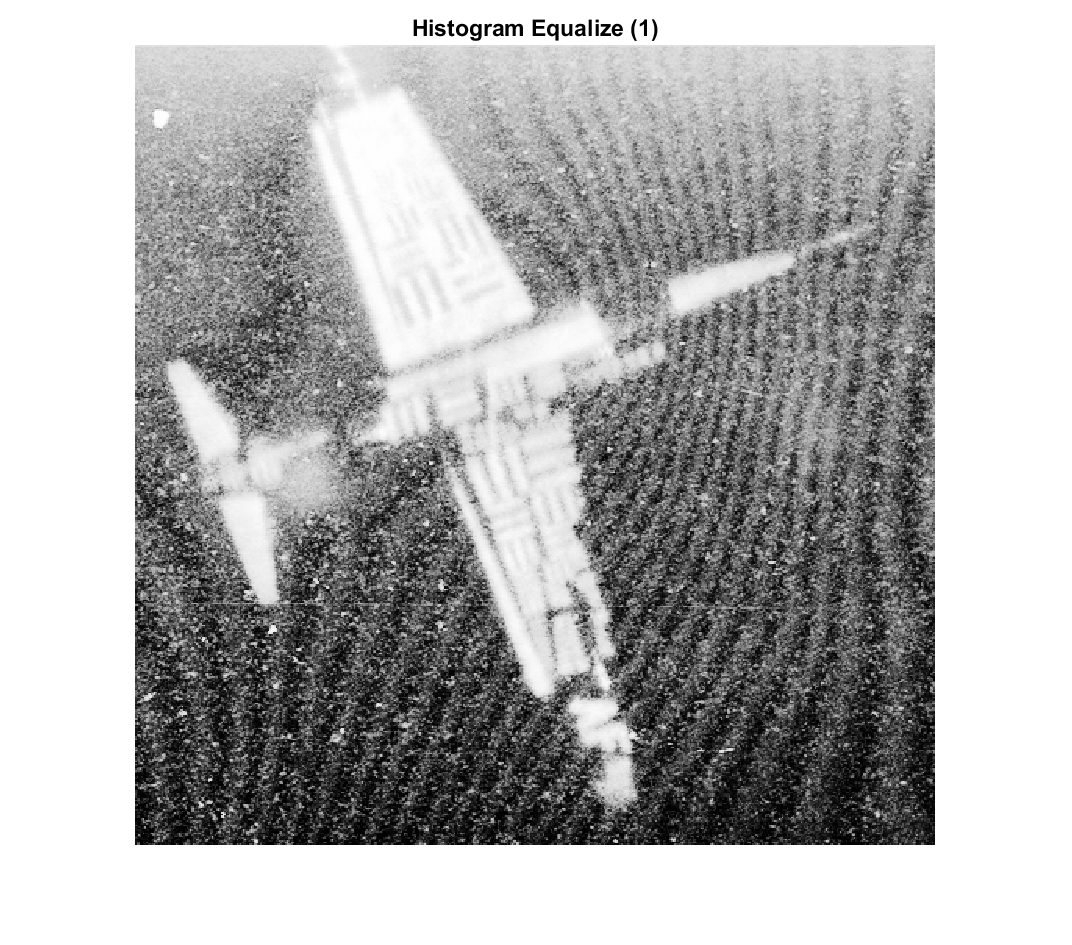
\includegraphics[width=0.5\columnwidth]{Histogram_Equalize_1.png}
\includegraphics[width=0.5\columnwidth]{Histogram_Equalize_2.png}

\pagebreak

\textbf{2.1.1 Q2 - Local Histogram Equalization}
\begin{verbatim}
function out = adaptive_histogram(img, H, W)
    out = img;
    img_height = size(img, 1);
    img_width = size(img, 2);
    for h_window = 1:H:img_height
        for w_window = 1:W:img_width
            if ((h_window + H - 1) > img_height)
                temp_H = img_height-h_window;
            else
                temp_H = H;
            end
            if ((w_window+H-1) > img_width)
               temp_W = img_width-w_window; 
            else
               temp_W = W;
            end
            out(h_window:h_window+temp_H-1,w_window:w_window+temp_W-1)=
            histogram_equalize(img(h_window:h_window+temp_H-1,w_window:w_window+temp_W-1));
        end
    end
end

imshow(adaptive_histogram(a, 100, 100));
imshow(adaptive_histogram(b, 200, 200));

\end{verbatim}
\includegraphics[width=0.5\columnwidth]{Adpative_Equalize_1.png}
\includegraphics[width=0.5\columnwidth]{Adpative_Equalize_2.png}

\pagebreak

\textbf{2.1.1 Q3 - Unsharp Mask}
\begin{verbatim}
function out = unsharp_mask(img, r, k)
    ind = (-r:r);
    [X Y] = meshgrid(ind, ind);
    sigma = r/3;
    h = exp(-(X.^2 + Y.^2) / (2*sigma*sigma)) / (2 * 3.14 * sigma.^2);
    h = h / sum(h(:));
    
    unsharp = img - spatial_filter(img, h);
    out = img + k*unsharp;
end

imshow(unsharp_mask(a, 5, 10));
imshow(unsharp_mask(b, 5, 5));

\end{verbatim}

\includegraphics[width=0.5\columnwidth]{Unsharp_Mask_1.png}
\includegraphics[width=0.5\columnwidth]{Unsharp_Mask_2.png}
\pagebreak

\textbf{2.1.1 Q4 - Laplacian Sharpening}
\begin{verbatim}
function out = laplacian_sharpen(img, k)
    img_double = im2double(img);
    laplacian = gradient(gradient(img_double));
    out = img + uint8(round(k*laplacian*255));
end

imshow(laplacian_sharpen(a, 8));
imshow(laplacian_sharpen(b, 20));

\end{verbatim}
\includegraphics[width=0.5\columnwidth]{Laplacian_Sharpen_1.png}
\includegraphics[width=0.5\columnwidth]{Laplacian_Sharpen_2.png}

\pagebreak

\textbf{2.1.1 Q5 Adaptive Histogram CLAHE}

\begin{verbatim}
function out = adaptive_histogram(img, H, W, cutoff)
    out = img;
    img_height = size(img, 1);
    img_width = size(img, 2);
    for h_window = 1:H:img_height
        for w_window = 1:W:img_width
            if ((h_window + H - 1) > img_height)
                temp_H = img_height-h_window;
            else
                temp_H = H;
            end
            if ((w_window+H-1) > img_width)
               temp_W = img_width-w_window; 
            else
               temp_W = W;
            end
            out(h_window:h_window+temp_H-1, w_window:w_window+temp_W-1)=
                histogram_equalize(img(h_window:h_window+temp_H-1,
                w_window:w_window+temp_W-1));
        end
    end
    before_cutoff = out;
    if nargin == 4
        if cutoff < (img_height * img_width / 255)
            disp ('invalid cutoff');
        else
            for pixel_val = 0:255
               count_pixels = length(before_cutoff(before_cutoff==pixel_val));
               if (count_pixels > cutoff)
                   mask = (before_cutoff==pixel_val);
                   for replace_count = 0:count_pixels-cutoff
                       ind = find(mask, 1, 'first');
                       mask(ind) = 0;
                       out(ind) = round(rand(1)*255);
                   end
               end
            end
        end
    end
end

imshow(adaptive_histogram(a, 100, 100, 2500));
imshow(adaptive_histogram(b, 200, 200, 1500));

\end{verbatim}

\includegraphics[width=1\columnwidth]{Adaptive_Equalize_CLAHE_1.png}

\includegraphics[width=1\columnwidth]{Adaptive_Equalize_CLAHE_2.png}

\pagebreak
\textbf{2.3.1}

For the additive and multiplicative noise, the image was first blurred with a Gaussian filter to reduce noise. It was then followed by a histogram equalization to deal with the low contrast issues. 


\includegraphics[width=0.5\columnwidth]{Additive_Noise.png}
\includegraphics[width=0.5\columnwidth]{Multiplicative.png}


For impulsive noise, the median filter was used as it removes outliers. Following that, a histogram equalize was used to improve the contrast.
\includegraphics[width=0.5\columnwidth]{Impulsive.png}

\pagebreak\pagebreak
The low contrast issue of the snowglobe was solved by increasing the overall brightness by adding '100' to the image. Afterwards, the image was contrast stretched, this resulted in an improved contrast for the image. To further enhance the image, a unsharp mask was applied to accentuate the edges.
\includegraphics[width=1\columnwidth]{Snowglobe.png}

\pagebreak

\end{document}
